\begin{frame}{Methodology: Agile Development Approach}
This project employed an \textbf{Agile development methodology} to handle evolving requirements through flexibility, collaboration, and iterative progress. Unlike traditional linear models, Agile embraces change via a continuous feedback loop with stakeholders.

To provide structure, the project was managed using \textbf{Scrum}, a popular and effective Agile framework.
\end{frame}

\begin{frame}{Scrum Roles}
\begin{itemize}
\item \textbf{Product Owner:} Key stakeholders at Infinity Datatech, primarily the Product Manager and technical leads, who defined the project vision and prioritized features based on organizational knowledge management needs.
\item \textbf{Development Team:} A self contained role filled by the developer on this academic project, responsible for building the full stack search engine system.
\item \textbf{Scrum Master:} A dual role fulfilled by the developer (process facilitation) and the academic supervisor (guidance and impediment removal).
\end{itemize}
\end{frame}

\begin{frame}{Scrum Artifacts}
\begin{itemize}
\item \textbf{Product Backlog:} A master list of all features and requirements, prioritized in collaboration with Infinity Datatech based on technical value and enterprise search needs.
\item \textbf{Sprint Backlog:} A subset of high priority tasks selected from the Product Backlog to be completed within a two week Sprint.
\item \textbf{Increment:} The tangible, working, and tested piece of software produced at the end of each Sprint, adding to previous functionality with deployable search components.
\end{itemize}
\end{frame}

\begin{frame}{Scrum Events}
The work was structured around recurring events within each two week Sprint:
\begin{enumerate}
\item \textbf{Sprint Planning:} Selecting items from the Product Backlog to define the Sprint Goal for search engine components.
\item \textbf{Daily Check-ins:} Brief, regular syncs to discuss progress and obstacles in development.
\item \textbf{Sprint Review:} A demonstration of the Sprint increment to Infinity Datatech stakeholders to gather critical feedback on search quality and system performance.
\item \textbf{Sprint Retrospective:} An internal reflection to identify process improvements for the next Sprint.
\end{enumerate}
\end{frame}

\begin{frame}{The Scrum Framework - Process Flow}
\begin{figure}
\centering
\begin{tikzpicture}[
scale=0.7,
artifact/.style={rectangle, draw, fill=orange!20, minimum height=0.8cm, minimum width=2cm, align=center, font=\tiny},
event/.style={rectangle, draw, fill=green!20, minimum height=0.7cm, minimum width=1.6cm, align=center, font=\tiny, rounded corners=0.3cm},
arrow/.style={->, thick},
sprint/.style={rectangle, draw, dashed, fill=gray!5, minimum height=2.5cm, minimum width=3.2cm}
]
% Top row - Planning phase
\node[artifact] (product_backlog) {Product\\Backlog};
\node[event, right=1.3cm of product_backlog] (sprint_planning) {Sprint\\Planning};
\node[artifact, right=1.3cm of sprint_planning] (sprint_backlog) {Sprint\\Backlog};
% Sprint box
\node[sprint, below=1.2cm of sprint_planning] (sprint_container) {};
\node[font=\bfseries, font=\tiny] at ([yshift=1cm]sprint_container.center) {2-Week Sprint};
\node[font=\tiny, align=center] at (sprint_container.center) {Daily Standups\\Development Work\\Collaboration};
% Bottom row - Review phase
\node[artifact, below=1.2cm of sprint_container] (increment) {Working\\Increment};
\node[event, left=1.3cm of increment] (sprint_review) {Sprint\\Review};
\node[event, right=1.3cm of increment] (retrospective) {Sprint\\Retrospective};
% Main flow arrows
\draw[arrow] (product_backlog) -- (sprint_planning);
\draw[arrow] (sprint_planning) -- (sprint_backlog);
\draw[arrow] (sprint_backlog) -- (sprint_container.north);
\draw[arrow] (sprint_container.south) -- (increment);
\draw[arrow] (increment) -- (sprint_review);
\draw[arrow] (increment) -- (retrospective);
% Feedback loops
\draw[arrow, bend left=25] (sprint_review) to node[above, font=\scriptsize] {Product Feedback} (product_backlog);
\draw[arrow, bend right=25] (retrospective) to node[below, font=\scriptsize] {Process Improvements} (sprint_planning);
\end{tikzpicture}
\caption{The Scrum Framework - Process Flow}
\label{fig:scrum_framework}
\end{figure}
\end{frame}

\begin{frame}{Project Management and Workflow Tools}
To support this Agile Scrum process, a specific set of digital tools was employed:
\begin{itemize}
\item \textbf{GitHub:} Used for version control and managing the \textbf{Product} and \textbf{Sprint Backlogs} via Projects and Issues features for tracking search engine development.
\item \textbf{Microsoft Teams:} Used for formal academic supervision meetings.
\item \textbf{Lark:} Serves as the central collaboration hub for daily communication, task tracking, and sprint management, coordinating distributed system components and data ingestion pipelines.
\end{itemize}
\end{frame}

\begin{frame}{Product Manager Interview - Requirements Discovery}
\scriptsize
\textbf{Example Q:} Can you describe the current challenges your technical teams face when searching for internal documentation?

\textbf{Outcome:}
\begin{itemize}
    \item Engineers spend 30-45 minutes daily searching across fragmented systems (Confluence, Google Drive, Git repositories, local shares).
    \item Existing keyword search misses conceptually related documents due to terminology variations.
    \item Critical visual information in charts and diagrams is not searchable, forcing manual document browsing.
    \item No unified interface, requiring context switching between multiple tools.
\end{itemize}

\vspace{0.5em}
\textbf{Example Q:} What types of queries do your teams typically need answers for?

\textbf{Outcome:}
\begin{itemize}
    \item Technical how-to questions requiring code examples and architecture diagrams.
    \item Troubleshooting queries needing logs, error messages, and past incident reports.
    \item Policy and compliance questions requiring exact citations from official documents.
    \item Comparative analysis requiring synthesis across multiple technical specifications.
    \item This revealed need for both precise retrieval and intelligent summarization.
\end{itemize}
\end{frame}

\begin{frame}{Product Manager Interview - Feature Priorities}
\scriptsize
\textbf{Example Q:} If you had to prioritize three capabilities for the search system, what would they be?

\textbf{Outcome:}
\begin{itemize}
    \item \textbf{Priority 1:} Multimodal search that can find documents based on visual content descriptions, not just text.
    \item \textbf{Priority 2:} Conversational interface where follow up questions refine results without starting over.
    \item \textbf{Priority 3:} Source attribution with exact citations so answers can be verified and trusted.
    \item Additional need: Sub-second query response time for daily usage adoption.
\end{itemize}

\vspace{0.5em}
\textbf{Example Q:} How do you currently evaluate whether search results are relevant?

\textbf{Outcome:}
\begin{itemize}
    \item Manual inspection of top 10 results for precision.
    \item User feedback on whether they found what they needed.
    \item Time to complete search task as efficiency metric.
    \item This informed our evaluation methodology using NDCG@10, MRR, and latency measurements.
\end{itemize}
\end{frame}

\begin{frame}{Workflow Analysis}
Detailed observations of Infinity Datatech manual search processes were conducted:
\begin{itemize}
    \item \textbf{Process mapping:} Documented the end to end workflow from query formulation to answer discovery, revealing an average of 7 context switches per search session across different data sources.
    \item \textbf{Time motion studies:} Measured time spent on manual tasks to identify bottlenecks. Average search session: 12 minutes, with 60 percent spent navigating between systems rather than evaluating content.
    \item \textbf{Artifact analysis:} Examined search logs and user feedback to understand information needs. Found 40 percent of queries require visual evidence and 65 percent benefit from conversational refinement.
    \item \textbf{Tool evaluation:} Assessed the current toolset (Confluence search, Google Drive search, file system grep) to find gaps. No system provided multimodal retrieval or intelligent ranking beyond keyword matching.
\end{itemize}
\end{frame}

\begin{frame}{Hierarchical Task Analysis}
The Hierarchical Task Analysis below outlines the system functional structure, decomposed into eight primary modules. This task breakdown forms the basis for the use cases and activity diagrams that follow.

\vspace{0.5em}
\begin{figure}
    \centering
    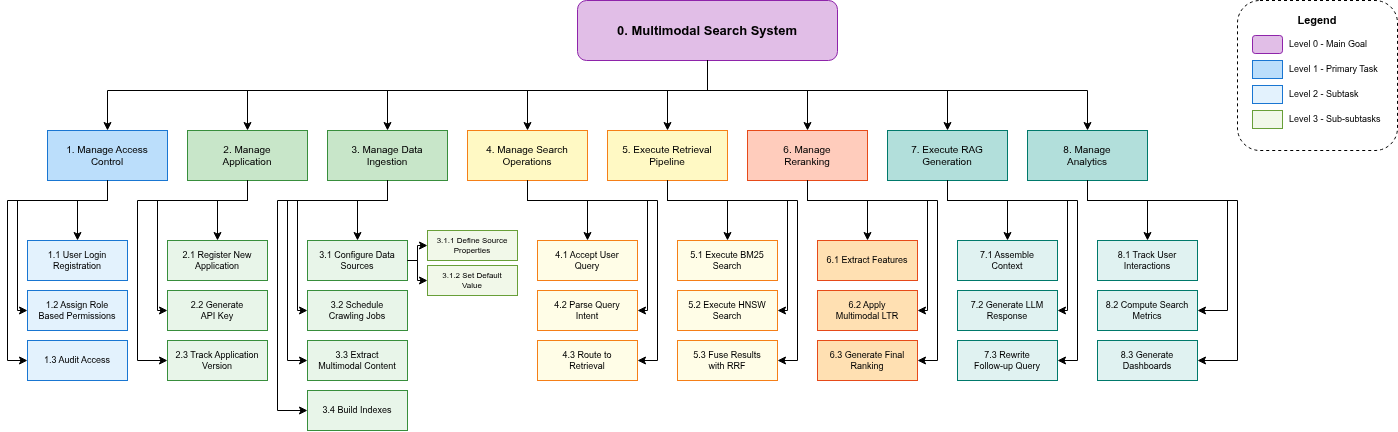
\includegraphics[width=0.95\textwidth]{HTA.drawio.png}
    \caption{Hierarchical Task Analysis of Verdant Search System}
    \label{fig:hta}
\end{figure}
\end{frame}

\begin{frame}{Stakeholder Introduction}
    \begin{columns}[t]
        \column{.48\textwidth}
        \textbf{Infinity Data Tech Sdn. Bhd.}
        \begin{itemize}
            \item Malaysian company specializing in VPN and AI customer service products
            \item Own application products and in house development
            \item Focus on software development and network protocol research
        \end{itemize}
        
        \column{.48\textwidth}
        \textbf{Project Context}
        \begin{itemize}
            \item Internal knowledge base search for technical teams
            \item Customer support documentation retrieval
            \item VPN technical knowledge and censorship circumvention expertise
        \end{itemize}
    \end{columns}
\end{frame}

\begin{frame}{System Architecture Overview}
    \begin{columns}[t]
        \column{.48\textwidth}
        \textbf{Backend Pipeline}
        \begin{itemize}
            \item Distributed web crawling with text and image extraction
            \item Dual indexing: Inverted index (BM25) + HNSW (CLIP embeddings)
            \item Compressed storage with incremental updates
            \item Two stage ranking: Fast retrieval + Multimodal LTR reranking
        \end{itemize}
        
        \column{.48\textwidth}
        \textbf{Frontend Interface}
        \begin{itemize}
            \item Dual panel UI: Document list + AI chat
            \item Conversational query refinement
            \item Real time result updates
            \item Closed loop: User follow up leads to query rewriting leads to new retrieval leads to updated AI response
        \end{itemize}
    \end{columns}
\end{frame}
